\documentclass[11pt, a4paper]{article}
\usepackage[english]{babel}
\usepackage{ragged2e}
\usepackage[utf8x]{inputenc}
\usepackage{amsmath}
\usepackage{float}
\usepackage{graphicx}
\usepackage[font=small,labelfont=bf]{caption}
\usepackage[top=1.0in, bottom=1.25in, left=1.20in, right=1.20in]{geometry}
\graphicspath{ {./Images/} }

\title{\vspace{-4cm}}
\author{}
\date{}

\begin{document}
\maketitle

\section{Literature Review / Background}

\subsection{Introduction}
This project is an attempt to combine multiple facets of game theory and artificial intelligence, in hope that the end result will be educational and/or useful to the fields. There are multiple stepping stones within the fields of game theory, mathematics, etc. which need to be examined in order to gain a further understanding of the project, which we will look at in this section.

\subsection{Brief History of Game Theory}
Game theory is the study of behaviours and mathematical models which result from the decisions and strategies of two or more economically rational players in either cooperative or non-cooperative strategy games. Applications of game theory have manifested in social science, psychology, mathematics and many more fields of study; however, the root interactions lie in strategic games such as the prisoner's dilemma or tit-for-tat. Game theory was introduced and popularised by mathematician John von Neumann, who first proved an optimal strategy for zero-sum games with perfect information such as chess or go called the minimax theorem in 1928. This theorem indicates that in such games, there is a pair of strategies for each player which allows them to minimise their maximum losses, while considering all responsive moves of the opponent. \\
\noindent
After von Neumann published his initial paper on game theory, he published a book co-authored by economist Oskar Morgenstein entitled, "Theory of Games and Economic Behaviour". Within this book, von Neumann fixates mainly on non-cooperative games and/or zero-sum games; but most importantly, identified a method of finding consistent solutions and strategies for both players in two-person zero-sum games. This work became a milestone for game theory as it established a foundation for becoming a unique discipline. \\
\noindent
Following this, numerous advancements in game theory occurred during the 1950s - mathematicians Merrill Flood and Melvin Dresher experimented mathematical and game versions of the prisoner's dilemma for the American think tank corporation, RAND (Research and Development). In the same year, John Forbes Nash Jr published his dissertation on non-cooperative games which contained the first definitions of the Nash equilibrium - an important milestone for adaptive strategy in game theory. He proved that in every n-player non-zero sum game, a Nash equilibrium existed, assuming the game had a finite number of actions. This was a continuation of the work from von Neumann and Morgenstein in their 1944 book, which only covered two person zero-sum games, and was restrained by the implications of 'rational' behaviour. \\
\noindent
In 1980, political scientist Robert Axelrod set up a multi-agent tournament for the iterated/repeated prisoner's dilemma. Multiple well-known game theorists from different professions such as psychology, political science, economics, mathematics and more submitted 14 FORTRAN (Formula Translation) programs for the agents to follow as implicit strategies. In this tournament, agents would play against each other for 200 rounds - mutual cooperation would yield 3 points, mutual defection 1 point, single defection 5 points and single cooperation 0 points. The winning strategy was a simple tit-for-tat program which cooperated on the first turn, then repeated the opponents previous move for each subsequent turn. This strategy ended the tournament with an average of 504.5 points of a maximum 1000. \\

\subsection{Prisoner's Dilemma}
The prisoner's dilemma is one of the fundamental games of game theory which shows the payoffs and consequences of two 'players' acting in their own self interests. This summary, cited from britannica.com, is a model version of the prisoner's dilemma: \\

\noindent
"\textit{Two prisoners are accused of a crime. If one confesses and the other does not, the one who confesses will be released immediately and the other will spend 20 years in prison. If neither confesses, each will be held only a few months. If both confess, they will each be jailed 15 years. They cannot communicate with one another. Given that neither prisoner knows whether the other has confessed, it is in the self-interest of each to confess himself. Paradoxically, when each prisoner pursues his self-interest, both end up worse off than they would have been had they acted otherwise.}" \\

\noindent
The first examples of the prisoner's dilemma being used in the context of game theory date back to the 1950s, by Merrill Flood and Melvin Dresher who devised puzzles and experiments using the structure of the dilemma - mainly an attempt to verify the usefulness of a non-cooperative Nash equilibrium. In this experiment, Flood and Dresher ran 100 games between two human players - in which player 1 (economist Armen Alchian) cooperated 68 times, while player 2 (mathematician John Williams) cooperated 78 times. In game theory, if a strategic game exists with the possibility for a various number of possible outcomes, a payoff matrix can be used to visually represent the benefits and consequences of each outcome. For the prisoner's dilemma, a typical payoff matrix would look as such:

\begin{figure}[h]
	\centering
		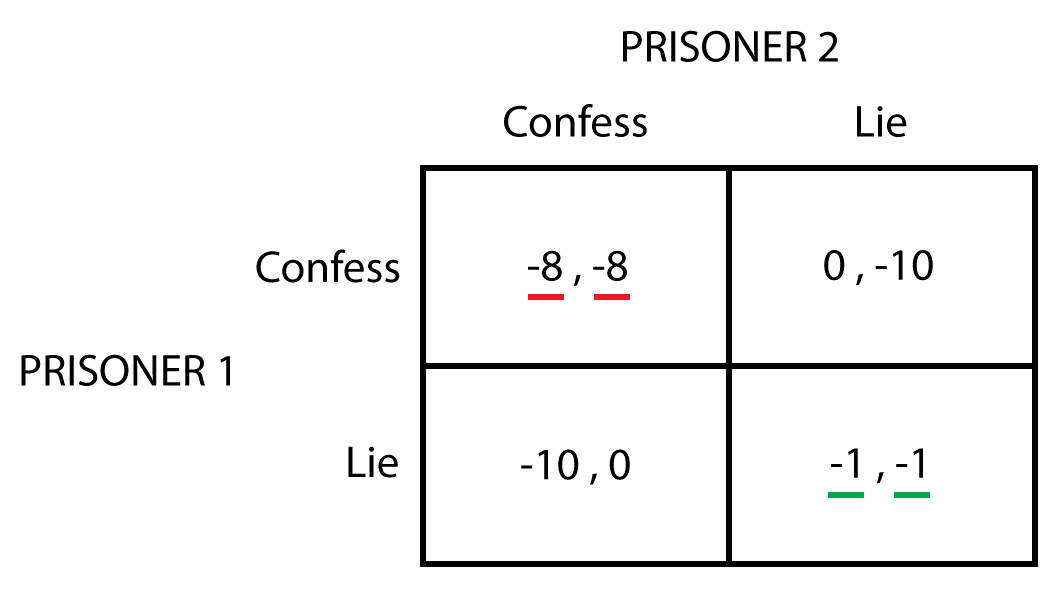
\includegraphics[width=0.6\textwidth]{DilemmaPayoffMatrix}
		\caption{Prisoner's Dilemma Payoff Matrix}
\end{figure}

\noindent
As you can see, the prisoner's would achieve the best possible equal payoff if they consistently chose to confess, but a prisoner could achieve a higher payoff if they were to follow their own self interests. However, the payoff matrix in this experiment looked like this:

\begin{figure}[H]
	\centering
		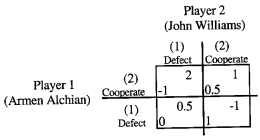
\includegraphics[width=0.5\textwidth]{FloodDresherPayoff}
		\caption{Flood-Dresher Experiment Payoff Matrix}
\end{figure}

\noindent
In the Flood-Dresher experiment, the restraints can be thought of as 'unfair' as human players have a level of empathy and other emotion which may sway their decision for reasons an A.I. program would never follow. Such an example would be the comments which player 1 made in their log of comments. Alchian, or player 1, wrote comments such as "He does not want to trick me. He is satisfied. I must teach him to share", while player 2 Williams wrote comments such as "A shiftless individual - opportunist, knave" (de Herdt, 2003, p. 189) just a turn apart from each other. Many economists, game theorists and mathematicians believe that the results of this experiment may have been swayed slightly due to each player being empathetic or vindictive at numerous points in the game. % needs more content

\subsection{Nash Equilibrium}
In 1950, John Forbes Nash Jr. published his dissertation entitled, "Non-cooperative Games". Within this dissertation was proof which indicated that within a two person zero-sum game, there exists an 'equilibrium point' for both players. This equilibrium was described in the paper as such, "Thus an equilibrium point is an n-tuple such that each player's mixed strategy maximizes his pay-off if the strategies of the others are held fixed. Thus each player's strategy is optimal against those of the others" (Nash, 1950, p. 3). Simply put, Nash was illustrating that within a two person game in which one player's benefit is a direct loss for the opponent, there lies a state in which neither player has any incentive to switch strategies, as it will not benefit their payoff - thus, the game sits at an equilibrium. The simplest, and most likely quickest way to prove the existence of a Nash equilibrium would be as follows:

\begin{figure}[H]
	\centering
		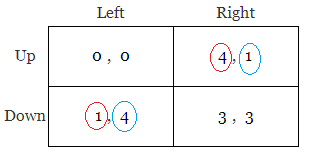
\includegraphics[width=0.5\textwidth]{ModelMatrix}
		\caption{Example Matrix}
\end{figure}

\noindent
Most proofs of equilibria exist if a certain number of conditions are met. Given a model payoff matrix, figure 3, our conditions for a pure/mixed strategy Nash equilibrium are as follows:

\begin{itemize}
  \item The first player's best response is the same against any potential move of the opponent (red circle).
  \item The second player's best response is the same against any potential move of the opponent (blue circle).
  \item Nash equilibrium = (Up, Right),(Down, Left).
\end{itemize}

\noindent
There are a few ways of proving the existence of a Nash equilibrium within games in a more detailed way - within Nash's dissertation, he chose to speak about the 'generalised' Kakutani fixed point theorem, and the Brouwer fixed point theorem.

\subsubsection{Kakutani's Fixed Point Theorem}
The Kakutani fixed point theorem states that a common fixed point exists within a collection of maps defined on non-empty, convex and compact subsets. Given the following scenario: \\

\noindent
\textit{"Let M be a compact, convex subset of Euclidean n-space. \footnote{A Euclidean space is sometimes known as n-space, and is simply the space of all n-tuples of real numbers.} Let T be a continuous set-valued function on M; i.e., a mapping from M to the set of all subsets of M, T→P(M). If T is such that T(x) is convex for all x belonging to M then there exists a z such that T(z) contains z."} (Kakutani, 1941, p. 457-459) \\

\noindent
This theorem can be proven if the following conditions are satisfied:

\begin{itemize}
  \item M is a non-empty, convex and compact set.
  \item T(x) is non-empty for all x ∈ M.
  \item For all x ∈ M, T(x) is a convex set.
  \item T(x) has a closed graph, i.e. if \{x\textsuperscript{n}, y\textsuperscript{n}\} → \{x, y\} with y\textsuperscript{n} ∈ T(x\textsuperscript{n}), then y ∈ T(x).
\end{itemize}

\noindent
If satisfied, a fixed point exists within T. \\

\noindent
The Kakutani theorem is a more generalised proof of the Brouwer fixed point theorem, but is used to prove a Nash equilibrium in a very similar way. The conditions used in both theorems can be modified in such a way that you would prove the existence of an equilibrium state rather than a fixed point, within a set of strategies rather than tuples. \\

\subsubsection{Applications of Nash equilibria}
Besides it's obvious magnitude in the fields of mathematics, Nash's work has had effects on fields such as computing, social science, psychology, and many more. Economists have used examples of the Nash equilibrium to calculate the prices of rival companies, predict prices of future products and calculate the best prices for supply and demand. A dissertation/report was published by the federal reserve bank of Minneapolis looking into why car insurance was so expensive in Philadelphia in the 90s, in which the writer chose to use a Nash equilibrium to demonstrate why the fluctuation of price was caused by the rivaling strategies of insurance providers. However, given the unpredictability of today's market, a Nash equilibrium may not have many uses outside of being a mathematical model in the field of economics. Another famous example would be the Cold War between the 40s and 90s - the USSR and the US were stuck in a long period of tension which could be seen as mutually assured destruction, in which each bloc knew the positions of the opponent but didn't start a war. This correlates exactly to a Nash equilibrium situation, where each side has no incentive to switch their strategy given the payoff. \\

\subsection{Repeated Games}
Repeated games, also known as iterated games or 'supergames' are either finitely or infinitely long games which repeat after finishing. These games are usually represented in extensive form, meaning each strategy and/or game is mapped out as a tree, with specific time-stamps for each game. Payoffs are included at the end of each branch. The main application and usefulness of repeated games is to examine how economically rational players may behave differently from game to game depending on previous strategies or moves. Arguably the most important instance of repeated games is Robert Axelrod's multi-agent tournament in 1980. This tournament was a simple 200 round prisoner's dilemma, in which mutual cooperation scored 3 points, mutual defection 1 point, single defection 5 points and single cooperation 0 points - with a 200 round maximum of 1000 points. Well known game theorists from multiple professions such as psychology, political science, economics, mathematics and sociology submitted FORTRAN (Formula Translation) programs which the agents would follow as strategies. The winning strategy was submitted by Professor Anatol Rapoport, which was a simple tit-for-tat program in which the agent would start with a cooperative choice, then mimic the opponent's choice on the previous turn. According to Axelrod in his primer, "This decision rule is probably the most widely known and most discussed rule for playing the Prisoner's Dilemma. It is easily understood and easily programmed" (Axelrod, 1980, p. 7). Interestingly, each participant of the tournament was made aware of the properties of the preliminary tournament, and thus, many of them made tit-for-tat programs which they tried to improve upon; but, the original and simple tit-for-tat program ended up performing better than the modified versions. \\
Within the tournament there were 3 strategies which were expected and known by the participants in advance - always defect, always cooperate, and random. A strategy in which the agent always defects is the safest strategy of any, and could be seen as a principle of game theory. However, although such a strategy is safe, there is a low chance of it being the best strategy due to it's 'no risk, no reward' drawback. The 'always cooperate' strategy performs well when matched against itself - as you can expect a maximum payoff, but when matched against a defecting opponent, there comes a minimum payoff. The 'random' strategy is simply cooperating 50\% of the time, in an attempt to reap the benefits of both strategies. This strategy is more of a utility for making sure the opponent's strategy accounts for all possibilities, but in the end the random strategy didn't perform well. Scores for these strategies can be seen in figure 4.

\begin{figure}[H]
	\centering
		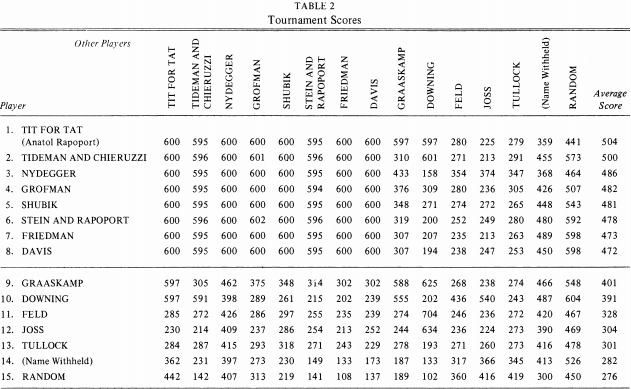
\includegraphics[width=0.7\textwidth]{AxelrodTournamentScores}
		\caption{Scores from the Axelrod Tournament}
\end{figure}

\noindent
\subsubsection{Folk Theorem}
Folk theorem is used within repeated games to show that a Nash equilibrium outcome in a game which is repeated infinitely is quantitatively and qualitatively equal and rational to that of a single game. While the origin of this theorem is unknown, it appeared in the 1950s and was quickly spread through the game theory field - thus the name, Folk Theorem. The first instance of a research paper to use the theorem was authored by James W. Friedman (1971) in his article, "Non-cooperative Equilibrium for Supergames", in which he details the payoffs of subgame-perfect \footnote{A subgame-perfect equilibrium means that if players were playing a smaller game which was part of a bigger game, their behaviour would represent a Nash equilibrium of that smaller game.} Nash equilibria in an infinitely repeated game, instead of using a single Nash equilibrium. This means that within a game such as the prisoner's dilemma, where mutual defection is a Nash equilibrium, folk theorem allows the possibility of a non-defection Nash equilibria in infinitely repeated games. Another important concept of folk theorem is that of duopolies and oligopolies; in an economic circumstance, a duopoly is a point in which two suppliers own all or nearly all of the market for a product or service. An oligopoly is the same, except the number of suppliers is more than 2 but remains a small number. When applied to the prisoner's dilemma, any choice other than mutual defection is unstable - however, if the games are infinitely repeated, there exists a possibility that one player may 'threaten' the other player to defect, in which case they would always play defect from that point onwards. In such a situation, if the second player is aware of this threat, they may choose to collude with their opponent and play cooperate, assuming there is a beneficial payoff guaranteed. In both economics and game theory, you can see a riskier, higher payoff as 'discounted' when colluding. % Needs more content?

\subsection{Machine Learning}
Machine learning is a subfield of articifical intelligence which combines pattern recognition and computational learning theory, an idea pioneered by Alan Turing in 1950, and developed by Arthur Samuel in 1959 through his paper, "Some Studies in Machine Learning Using the Game of Checkers''.\footnote{While some may argue that Marvin Minsky pioneered the first instance of a self-learning machine in 1951, many still question whether or not this project was artificial intelligence, given the amount of missing information.} The main goal of machine learning is for algorithms to become `smarter' on each iteration of instructions, such as a move in a game of checkers, to then make predictions based on the data it has constructed. Within Samuel's introduction to his paper, he states, "The studies reported here have been concerned with the programming of a digital computer to behave in a way which, if done by human beings or animals, would be described as involving the process of learning" (Samuel, 1959, p. 1). Samuel's checkers algorithm used a search tree to identify each of the board positions reachable from the available pieces\footnote{Samuel described this process as `looking ahead a few moves' like a human player might do.}, which would feed into a scoring algorithm - incorporating von Neumann's minimax strategy to choose the best move. The result of this algorithm, through rigorous testing, was a piece of artificial intelligence which could, "greatly outperform an average person'', and was envisioned to be economically viable in real-life situations/problems. This is the first instance of an algorithm which has developed itself without being given information directly.


\clearpage

\end{document}